\section{Barcode}
The barcode is a visual representation of the amount of plagairism in each page of the target document. In our application it is used in two representations, which use the same data source but have another visual layout and details shown within.

The barcode has 4 different colors, which represent another amount of plagairism within the page:

\begin{itemize}
\item      light blue: the page is disabled for the barcode
\item      white: page not available or no plagiarism
\item      black: more than 0 percent plagiarized
\item      dark red: more than percent plagairized
\item      light red: more than percent plagairized
\end{itemize}

\textbf{Representation with labels on the home page}

The first representation can be found at the home page, here are the barcodes of all published cases being displayed. The barcode is being displayed with page numbers below and the width is dynamic, so the barcode increases when the page gets wider and the barcode gets smaller, when the page width decreases. 

\begin{figure}[!h]
  \centering
  \fbox{
    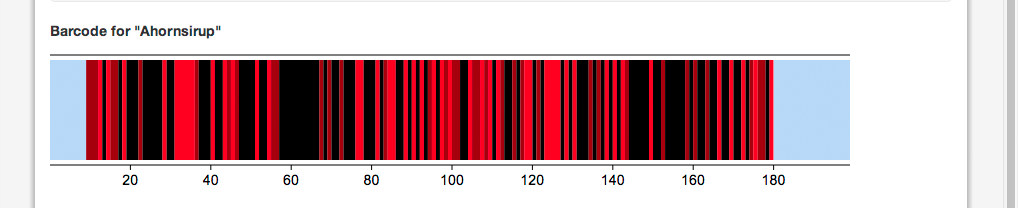
\includegraphics[width=0.97\textwidth]{images/feature-barcode-website.png}
  }
  \caption{Barcode on home page}
  \label{fig:feature-barcode-website}
\end{figure}

Since this mechanism is very dynamic, an algorithm needed to be developed to calculate the x axis values taking into consideration the page width and the number of pages in the document being visualized. It assumes that a label needs at least 45px of width and the whole barcode has to look well to a width of 500px.

So what we do is, we start with a setpsize of 10 for the page numbers: 10 20 30 40 50, now we check if the amount of pages can be displayed with such a fine scale to stay in the 500px range. For example a page count of 200 leeds to 20 values on the x axis and if we assume 45px are necessary to display a value on the axis properly, we would need 900px of width, but we have only 500px available. Otherwise we would have crossovers when we get below 900px. So the stepsize is increased by 10, until we stay in the 500px maximum width. As it turns out, a step size of 20 pages is sufficent to get a width of 450px in the end. The code for this calculation is being shown below.

\begin{lstlisting}[caption=Generating the barcode x axis]
private function generateAxis() {
        $labelStepsize = 10;

        while (true) {
            $count = sizeof($this->pages);
            $labelCount = floor($count / $labelStepsize);

            // we assume a label needs 45px and 500px is the width that needs to be displayable without crossovers
            if (45 * $labelCount > 500) {
                $labelStepsize += 10;
                continue;
            }
            break;
        }

        $label = $labelStepsize;
        $x = 0;
        while ($x < ($this->width - ($this->initWidth * $labelStepsize))) {
            $x += ($this->initWidth * $labelStepsize);
            $this->result .= '<text x="' . $x . $this->widthUnit . '" y="' . $this->y . '" font-family="Arial" font-size="14" text-anchor="middle">' . $label . '</text>';
            $this->result .= '<line x1="' . $x . $this->widthUnit . '" y1="' . ($this->y - 20) . '" x2="' . $x . $this->widthUnit . '" y2="' . ($this->y - 15) . '" stroke-width="1" stroke="#000000"></line>';

            $label += $labelStepsize;
        }
    }
\end{lstlisting}

\textbf{Representation without labels in the report}

The second area where barcodes are used, are the final reports. They will be explained in the next section. The space available in the PDF is much less than on the website and the library we are using for generating the PDF report does not support text in scable vectors graphics, so we decided to display the barcodes without labels for now. However the data visualized is exactly the same.